\subsection{Lines of Code within the Kuadrant Project}
An overall size of the Kuadrant project is required to know how much effect the cyclomatic complexity has over the project.
The first chat, \textbf{Figure \ref{fig:project_loc}}, is interesting as it shows the LoC\footnote{lines of code} for every repo.
It is interesting to see how and where the Kuadrant project grow over time.

\begin{figure}
	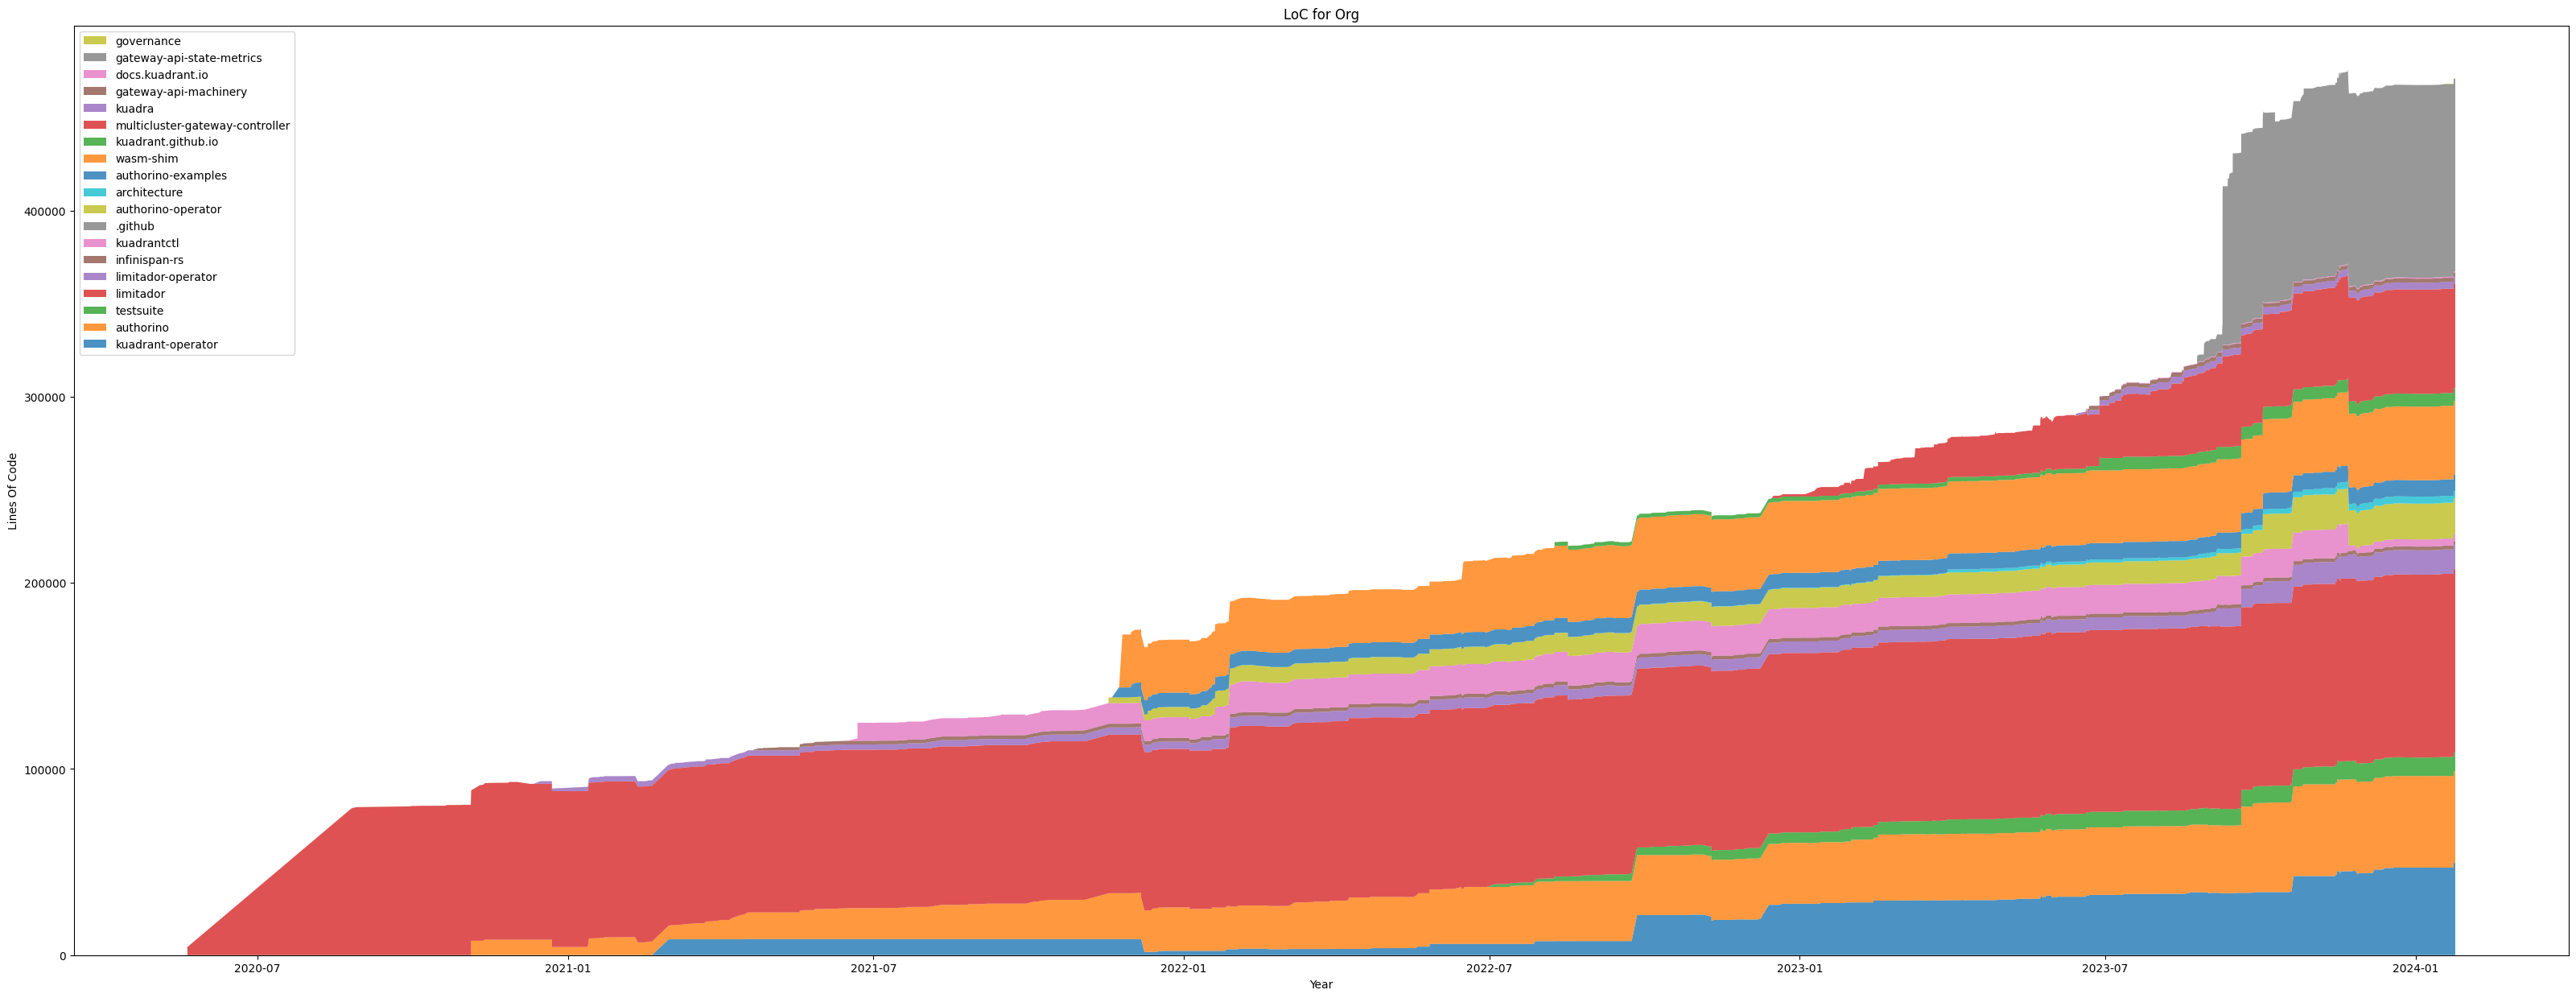
\includegraphics[width=\textwidth]{project_loc.png}
	\caption{Lines of code for all Kuadrant projects.}
	\label{fig:project_loc}
\end{figure}

Now to see the amount of the project code base that was scanned by the cyclomatic complexity tools, \textbf{Figure \ref{fig:project_scanned_loc}}.

\begin{figure}
	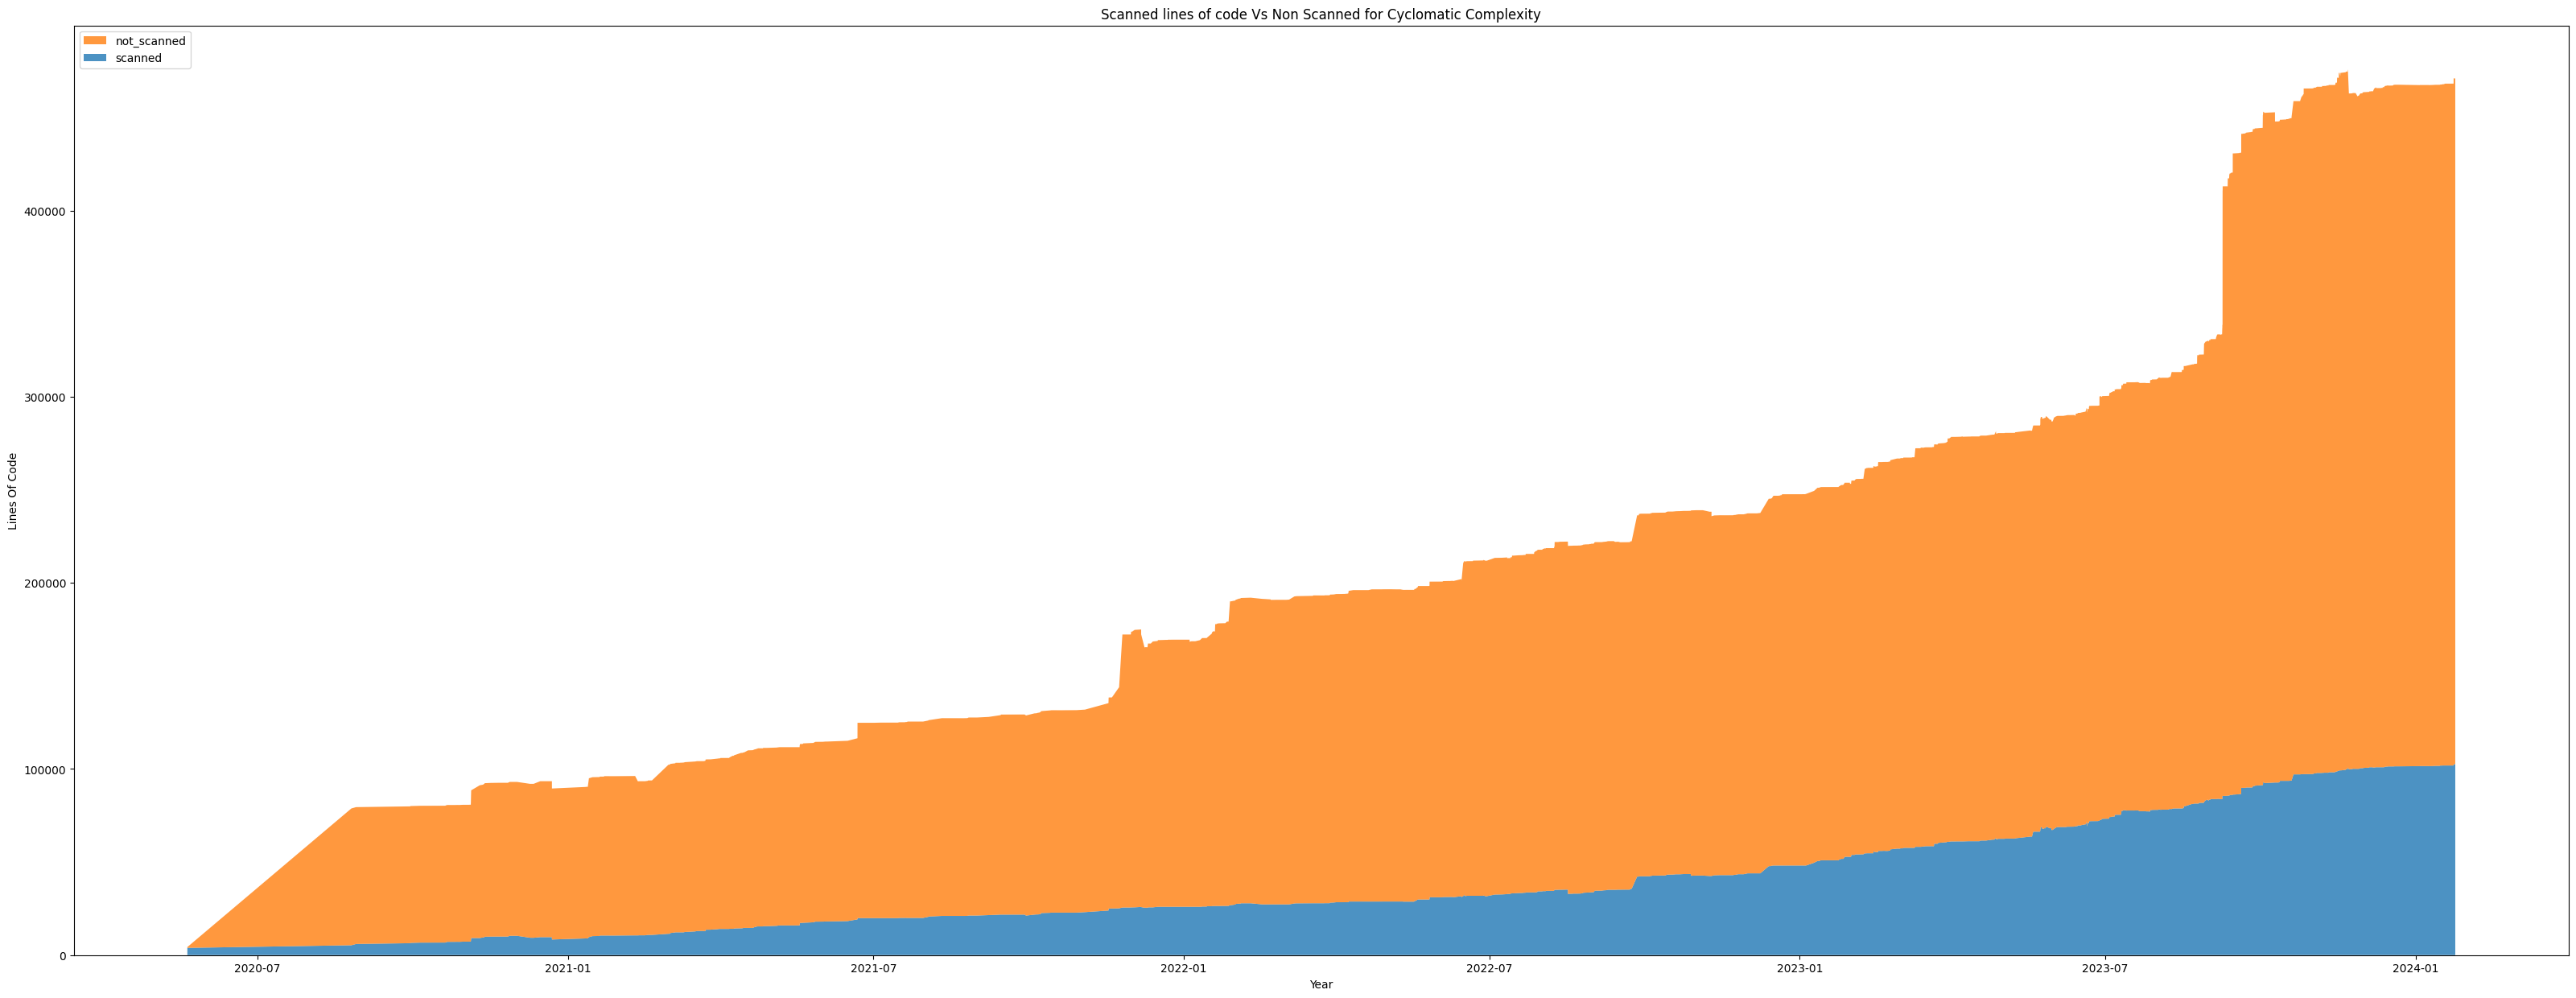
\includegraphics[width=\textwidth]{project_scanned_loc.png}
	\caption{Lines of code in the Kuadrant projects scanned by the cyclomatic complexity tools.}
	\label{fig:project_scanned_loc}
\end{figure}

As seen there is a very small amount of the LoC covered by the scan tools.
A lot of the projects are for working on kubernetes which relies heavily on YAML which we generate.
This could be a good explanation for the differences.
The one thing to note on the scannable code is the rate of change over time, while always increasing there are no steep increases.

